%==========================================
%
% Sibgrapi 2019 paper template
% Example of IEEEtran.cls
%
%==========================================

% *** Authors should verify (and, if needed, correct) their LaTeX system  ***
% *** with the testflow diagnostic prior to trusting their LaTeX platform ***
% *** with production work. The IEEE's font choices and paper sizes can   ***
% *** trigger bugs that do not appear when using other class files.       ***                          ***
% The testflow support page is at:
% http://www.michaelshell.org/tex/testflow/
%\documentclass[draftcls,onecolumn,12pt]{IEEEtran}

\documentclass[10pt,conference,pdftex]{IEEEtran}
\usepackage{todonotes}

% Some very useful LaTeX packages include:
% (uncomment the ones you want to load)


% *** MISC UTILITY PACKAGES ***
%
%\usepackage{ifpdf}
% Heiko Oberdiek's ifpdf.sty is very useful if you need conditional
% compilation based on whether the output is pdf or dvi.
% usage:
% \ifpdf
%   % pdf code
% \else
%   % dvi code
% \fi
% The latest version of ifpdf.sty can be obtained from:
% http://www.ctan.org/pkg/ifpdf
% Also, note that IEEEtran.cls V1.7 and later provides a builtin
% \ifCLASSINFOpdf conditional that works the same way.
% When switching from latex to pdflatex and vice-versa, the compiler may
% have to be run twice to clear warning/error messages.






% *** CITATION PACKAGES ***
%
\usepackage{cite}
% cite.sty was written by Donald Arseneau
% V1.6 and later of IEEEtran pre-defines the format of the cite.sty package
% \cite{} output to follow that of the IEEE. Loading the cite package will
% result in citation numbers being automatically sorted and properly
% "compressed/ranged". e.g., [1], [9], [2], [7], [5], [6] without using
% cite.sty will become [1], [2], [5]--[7], [9] using cite.sty. cite.sty's
% \cite will automatically add leading space, if needed. Use cite.sty's
% noadjust option (cite.sty V3.8 and later) if you want to turn this off
% such as if a citation ever needs to be enclosed in parenthesis.
% cite.sty is already installed on most LaTeX systems. Be sure and use
% version 5.0 (2009-03-20) and later if using hyperref.sty.
% The latest version can be obtained at:
% http://www.ctan.org/pkg/cite
% The documentation is contained in the cite.sty file itself.






% *** GRAPHICS RELATED PACKAGES ***
%
%\ifCLASSINFOpdf
  %\usepackage[pdftex]{graphicx}
  % declare the path(s) where your graphic files are
\graphicspath{{figs/}}
  % and their extensions so you won't have to specify these with
  % every instance of \includegraphics
\DeclareGraphicsExtensions{.pdf,.jpeg,.png,.jpg}
%\else
  % or other class option (dvipsone, dvipdf, if not using dvips). graphicx
  % will default to the driver specified in the system graphics.cfg if no
  % driver is specified.
   %\usepackage[dvips]{graphicx}
  % declare the path(s) where your graphic files are
%   \graphicspath{{../figs/}}
  % and their extensions so you won't have to specify these with
  % every instance of \includegraphics
   %\DeclareGraphicsExtensions{.eps}
%\fi
% graphicx was written by David Carlisle and Sebastian Rahtz. It is
% required if you want graphics, photos, etc. graphicx.sty is already
% installed on most LaTeX systems. The latest version and documentation
% can be obtained at:
% http://www.ctan.org/pkg/graphicx
% Another good source of documentation is "Using Imported Graphics in
% LaTeX2e" by Keith Reckdahl which can be found at:
% http://www.ctan.org/pkg/epslatex
%
% latex, and pdflatex in dvi mode, support graphics in encapsulated
% postscript (.eps) format. pdflatex in pdf mode supports graphics
% in .pdf, .jpeg, .png and .mps (metapost) formats. Users should ensure
% that all non-photo figures use a vector format (.eps, .pdf, .mps) and
% not a bitmapped formats (.jpeg, .png). The IEEE frowns on bitmapped formats
% which can result in "jaggedy"/blurry rendering of lines and letters as
% well as large increases in file sizes.
%
% You can find documentation about the pdfTeX application at:
% http://www.tug.org/applications/pdftex





% *** MATH PACKAGES ***
%
\usepackage[cmex10]{amsmath}
% A popular package from the American Mathematical Society that provides
% many useful and powerful commands for dealing with mathematics.
%
% Note that the amsmath package sets \interdisplaylinepenalty to 10000
% thus preventing page breaks from occurring within multiline equations. Use:
\interdisplaylinepenalty=2500
% after loading amsmath to restore such page breaks as IEEEtran.cls normally
% does. amsmath.sty is already installed on most LaTeX systems. The latest
% version and documentation can be obtained at:
% http://www.ctan.org/pkg/amsmath
\usepackage{amsthm}
\newtheorem{definition}{Definition}

\usepackage{gensymb}

% *** SPECIALIZED LIST PACKAGES ***
%
\usepackage{algorithmic}
% algorithmic.sty was written by Peter Williams and Rogerio Brito.
% This package provides an algorithmic environment fo describing algorithms.
% You can use the algorithmic environment in-text or within a figure
% environment to provide for a floating algorithm. Do NOT use the algorithm
% floating environment provided by algorithm.sty (by the same authors) or
% algorithm2e.sty (by Christophe Fiorio) as the IEEE does not use dedicated
% algorithm float types and packages that provide these will not provide
% correct IEEE style captions. The latest version and documentation of
% algorithmic.sty can be obtained at:
% http://www.ctan.org/pkg/algorithms
% Also of interest may be the (relatively newer and more customizable)
% algorithmicx.sty package by Szasz Janos:
% http://www.ctan.org/pkg/algorithmicx




% *** ALIGNMENT PACKAGES ***
%
\usepackage{array}





% *** SUBFIGURE PACKAGES ***
\ifCLASSOPTIONcompsoc
  \usepackage[caption=false,font=normalsize,labelfont=sf,textfont=sf]{subfig}
\else
  \usepackage[caption=false,font=footnotesize]{subfig}
\fi






% *** PDF, URL AND HYPERLINK PACKAGES ***
%
\usepackage{url}
% correct bad hyphenation here
\hyphenation{op-tical net-works semi-conduc-tor}
\usepackage[normalem]{ulem}

\begin{document}
%
% paper title
% Titles are generally capitalized except for words such as a, an, and, as,
% at, but, by, for, in, nor, of, on, or, the, to and up, which are usually
% not capitalized unless they are the first or last word of the title.
% Linebreaks \\ can be used within to get better formatting as desired.
% Do not put math or special symbols in the title.
\title{Equirectangular Image Quality Assessment Tool Integrated into the Unity Editor}

%-------------------------------------------------------------------------
% change the % on next lines to produce the final camera-ready version
\newif\iffinal
\finalfalse
%\finaltrue
\newcommand{\cmtid}{99999}
%-------------------------------------------------------------------------

% author names and affiliations
% use a multiple column layout for up to two different
% affiliations

\iffinal

% author names and affiliations
% use a multiple column layout for up to three different
% affiliations
\author{\IEEEauthorblockN{Adriano Gil}
\IEEEauthorblockA{SIDIA instituto de Tecbologia\\
Manaus, Brazil\\
Email: adriano.gil@sidia.com}
\and
\IEEEauthorblockN{Aasim khurshid}
\IEEEauthorblockA{SIDIA instituto de Tecbologia\\
Manaus, Brazil\\
Email: aasim.khurshid@sidia.com}
\and
\IEEEauthorblockN{Juliana Postal}
\IEEEauthorblockA{SIDIA instituto de Tecbologia\\
Manaus, Brazil\\
Email: juliana.postal@sidia.com}
\and
\IEEEauthorblockN{Thiago Figueira}
\IEEEauthorblockA{SIDIA instituto de Tecbologia\\
Manaus, Brazil\\
Email: thiago.figueira@sidia.com}
}

% conference papers do not typically use \thanks and this command
% is locked out in conference mode. If really needed, such as for
% the acknowledgment of grants, issue a \IEEEoverridecommandlockouts
% after \documentclass

% for over three affiliations, or if they all won't fit within the width
% of the page, use this alternative format:
%
%\author{\IEEEauthorblockN{Michael Shell\IEEEauthorrefmark{1},
%Homer Simpson\IEEEauthorrefmark{2},
%James Kirk\IEEEauthorrefmark{3},
%Montgomery Scott\IEEEauthorrefmark{3} and
%Eldon Tyrell\IEEEauthorrefmark{4}}
%\IEEEauthorblockA{\IEEEauthorrefmark{1}School of Electrical and Computer Engineering\\
%Georgia Institute of Technology,
%Atlanta, Georgia 30332--0250\\ Email: see http://www.michaelshell.org/contact.html}
%\IEEEauthorblockA{\IEEEauthorrefmark{2}Twentieth Century Fox, Springfield, USA\\
%Email: homer@thesimpsons.com}
%\IEEEauthorblockA{\IEEEauthorrefmark{3}Starfleet Academy, San Francisco, California 96678-2391\\
%Telephone: (800) 555--1212, Fax: (888) 555--1212}
%\IEEEauthorblockA{\IEEEauthorrefmark{4}Tyrell Inc., 123 Replicant Street, Los Angeles, California 90210--4321}}

\else
  \author{Sibgrapi paper ID: \cmtid \\ }
\fi


% make the title area
\maketitle

% As a general rule, do not put math, special symbols or citations
% in the abstract
\begin{abstract}\label{sec:abstract}
Virtual Reality (VR) applications provide an immersive experience when using panoramic images that contain a 360-degree view of the scene. Currently, the equirectangular image format is the widely used pattern to represent these panoramic images. The development of 360-degree images in the equirectangular image format, however, is under the influence of several parameters that define the quality of the captured image. Such parameters include resolution configurations, texture-to-objects mappings and deciding from different media formats, but to select the optimal value of these parameters, visual quality analysis is required. In this work, we propose a tool integrated within Unity editor to automate this quality assessment using different settings for the visualization of the 360-degree images. We compare the texture mapping of a skybox with a procedural sphere and a cubemap using the objective metrics for Image Quality Analysis (IQA). Based on the assessment results, the tool decides how the final image will be rendered at the target device to produce to produce a visually pleasing and high-quality image.
\end{abstract}

% no keywords

% For peerreview papers, this IEEEtran command inserts a page break and
% creates the second title. It will be ignored for other modes.
\IEEEpeerreviewmaketitle

\section{Introduction} \label{sec:introduction}
Images captured in the 360-degree surroundings of a single point are capable of replicating the entire visual information available from that position. Specific cameras are designed to capture such images as the Samsung Gear 360\degree, which captures panoramic images and stores them in a suitable format for 360-degree visualization. These images are stored in a specific format to facilitate image processing. The equirectangular format is the most common one. Furthermore, equirectangular images are used in Virtual Reality applications to provide an immersive user experience and allow users to explore the virtual environment from a first-person perspective. \par

Virtual Reality (VR) devices render the virtual world using a different image for each eye in order to emulate depth and as a result, increase the sense of presence within the context of the application. Although the technology behind the VR headset display has evolved, it still faces the challenge of offering a high density of pixels per Field of View (FoV) degree. Furthermore, the human eye has an estimated resolution of 60 pixels per degree, which means that an average 100-degrees device should render its content at a 6k resolution to provide realistic spatial emulation~\cite{va1965visual}. \par

A 360-degree image viewer usually renders its contents in a sphere to mimic the natural placement of visual elements as they would be perceived by the user in the real world. A large number of pixels are required to keep the quality of the pictures. The research for the best possible visual quality means picking an exhibition format in a given set of different exhibition formats, each one with different distortion degrees along the existing 360 degrees. To decide the appropriate format and resolution for a 360-degree image, it is necessary to take into consideration the device in which this picture will be displayed.
Therefore, an image quality assessment tool should have the ability to simulate devices and compare different quality settings to provide the most suitable image choice.\par

There are two approaches for image quality assessment: subjective and objective metrics. Subjective Image Quality Analysis (IQA) employs human observers to evaluate and score a sequence of pictures whereas Objective IQA builds mathematical models for automatic image quality assessment. Subjective IQA is accurate, but it is expensive and time-consuming. On the other hand, objective IQA may provide a cost-effective solution for image analysis and can be embedded in VR applications. To build VR applications, various tools have been proposed such as Unity Editor, Source and Panda3D to name a few. \par

Unity Editor is a game development engine for computers, mobile, console, virtual and augmented reality. It is both used by small development groups as well as big corporations such as Microsoft; it is also the most used development tool for virtual reality. From its GitHub account\footnote{https://github.com/Unity-Technologies/SkyboxPanoramicShader}, Unity provides built-in solutions for rendering panoramic images. The developer is also able to create customized solutions through shaders, i.e., code that is executed in the GPU and influences how 3D elements are displayed on the device screen.

In this paper, we propose an equirectangular image quality assessment tool which employs objective metrics integrated into the Unity Editor. To make assessments close to real case scenarios, our tool is capable of simulating visualization with the field of view and resolution values provided by the user. Figure~\ref{fig:tool} below presents the Unity Editor interface we built. By configuring specific values for the field of view and screenshot (image) resolution, it is possible to simulate the viewport of a given device. For instance, a 101-degree field of view and 1440 x 1480 resolution is close to the user view inside a VR application running on a Samsung S9 device. The screenshot direction field lets the user insert three-dimensional vectors indicating the direction each screenshot will be pointing to. Finally, a report and graphs are generated according to the chosen metrics.

\begin{figure}[ht!]
    \centering
    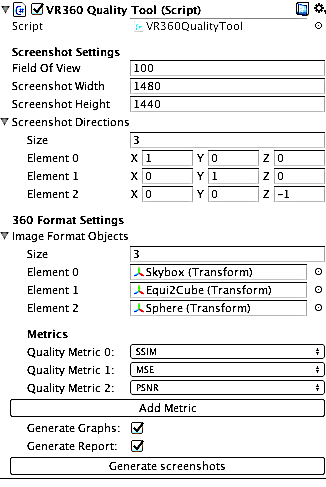
\includegraphics[width=0.73\linewidth]{figs/tool_edit.png}%
    \caption{Proposed tool embedded in Unity interface.}
    \label{fig:tool}
\end{figure}


The rest of the paper is organized as follows: Section~\ref{sec:related_work} reviews the most relevant work in equirectangular images and IQA. Next, the proposed method is detailed in Section~\ref{sec:proposedMethod}. Furthermore, the preliminary experimental results are presented and discussed in Section~\ref{sec:experiments}. Finally, conclusions and future work perspectives are given in Section~\ref{sec:conclusion}.

\section{Related Work}\label{sec:related_work}

VR applications differ from other vision applications due to their innate concern to provide content to all possible VR viewpoints. Furthermore, VR headsets can isolate the spectator both visually and acoustically from the real world~\cite{fuchs2017virtual}.
Spherical panoramic content may be presented in different projection types: equirectangular (ERP), rectilinear, doughnut, cube-map, and multiview~\cite{zakharchenko2016quality}. Moreover, the format of the 360-degree image plays a vital role in the resolution and uniformity of such images~\cite{dunn2017resolution}. For example, equirectangular images have a high resolution on the poles and high uniformity on the equator line; On the other hand, cube-map images have a high density on the edges and high uniformity in each face of the diagonal~\cite{duanmu:2018}. For all these projection types, the quality of the images selected to create a panoramic view is crucial to present the panoramic content.  \par

Image Quality Analysis (IQA) assesses the quality of the images in the creation of panoramic view. IQA is categorized into two types, i.e., subjective analysis and objective analysis~\cite{wang2006modern}. The most reliable strategy to evaluate image quality is through subjective analysis. In this case, human observers assess a set of pictures and score it on a scale from 1 (worst) to 5 (best), this technique is called MOS (Mean Opinion Score) and it calculates the average score given a set of scores for each sample. Pinson et al. compared and analyzed various methodologies for subjective video quality assessment~\cite{pinson:2003}. These test methods include single or double stimulus methods. In single stimulus methods, only one impaired video stream is used for assessment. In double stimulus, however, a reference videos is also provided to the user for comparative analysis~\cite{pinson:2003}.  \par

Although subjective IQA  methods are precise, they are inconvenient and expensive, especially when a VR environment is evaluated because it is more immersive. Thus, a complementary objective metric would be useful and less expensive. Objective metrics are defined as Full-Reference (FR), No-Reference (NR), and Reduced-Reference (RR)~\cite{li:2019}. In FR-IQA methods, a non-distorted reference image is available to evaluate the test image. In RR-IQA methods, a reference image with only selective information is available to compare and measure the quality of the distorted image. Whereas in NR-IQA methods, there is no reference image available to compare, the only image available is the one in which quality is measured.\par

Prior work on 360-degree IQA is discussed in Quality metric for spherical panoramic video~\cite{zakharchenko2016quality}. In this work, we focus on Full-reference IQA. Recent advancements in FR-IQA methods are comprehensively discussed in FR stereo image quality assessment using natural stereo scene statistics~\cite{md2015full}.  We propose an FR quality assessment tool for the selection of images before using them to render on the target device. Despite our focus on image quality assessment of 360-degree spherical panoramic images, our proposal only assesses screenshots obtained from texture projections inside Unity3D. Therefore, our final target are 2D images as a result of such projections; which is intuitive because still 360-degree images or video-sequences are encoded and transmitted in the 2D format under sphere-to-plane projection.
% \par \textcolor{red}{REVIEWED} \par
% \todo{The proposed method starts from here???}
% \textcolor{red}{THERE SHOULD BE A SECTION SAYING "THE PROPOSED METHOD" and all the details about the method should go there.. it is principal at this point. For now, it seems like there is something going on, but its not possible to understand what is going on...
% \\ \\ Also, I labeled the sections above this, I am not sure from where the proposed methodology starts and stuff, If you create sections, please label them as well. Same for figures, tables etc. So if we need to cross reference anything it would be correct. Hard quoted references can create problems in the future if we change the order of the image or section or whatever. The conventions I use for labeling sections is "sec:sectionName", Figures "fig:figurelabel" and for tables "tab:tableName".. We can use this or if you have some other convention, but we should follow a pattern, that would be nice. \\ \\
% Also, instead of naming the figures, screenshot-xxxx---xxx. We can name better that explains atleast a bit of context of the figure. }

\section{Proposed Method}\label{sec:proposedMethod}

% General proposal
In this work, we propose a full-reference objective IQA tool to analyze viewport-based patches of panoramic images. Our implementation runs as a customs inspector script in Unity that mimics how the final image is going to be rendered at the target device. Different rendering implementations can be tested using the same equirectangular image. We also describe our implementation of converting an equirectangular image into a cubemap format.

% FR IQA metrics / Skybox
Our solution is a fully-automatic way to compare different rendering configurations of spherical images. After choosing an equirectangular image, a target resolution, a field of view in degrees, a set of viewing directions and a set of rendering solutions, different images patches are generated according to an approximated viewport inside the panoramic exhibition. Each image patch is evaluated according to objective metrics using a reference patch. In order to compare different rendering implementations, we chose Skybox rendering as the reference image, considering its widespread usage in game and virtual reality applications.

% Conversion among different rendering approaches
The standard implementation of a spherical image viewer makes use of a sphere with inverted normals. Due to their characteristics, equirectangular images are distorted at poles, while cubemaps are distorted at their corners \cite{dunn2017resolution}. That is why it is interesting to test an image in different formats. In this section, we describe a shader-based implementation to fit equirectangular images in a cubemap visual representation.

% Paper structure

\subsection{Projecting 360\degree Images to UV Mapping} \label{sec:uvmapping}

Panoramic images comprehend the entire field-of-view of the user. Considering the
equirectangular format, some mapping implementations are listed below:

\begin{enumerate}
    \item Utilize a sphere mesh to render the 360-degree image inside it;
    \item Utilize a Skybox to render the 360-degree image on the background;
    \item Map the 360-degree image to UV positions of a cubic mesh.
\end{enumerate}

Each mapping possibility has its advantages and disadvantages in terms of resolution offered by angular direction and general distortion of the 360-degree image.

\subsection{Mapping Equirectangular Images to a Sphere}

For mapping equirectangular images to sphere, we adopt the standard UV mapping technique for spheres which is based on the latitude/longitude approach. That means we need to find a three-dimension coordinate ($x$, $y$, $z$) for a set of $n x m$ UV coordinates ($u$,$v$).

Given $n$ longitude values, the angular size $T$ can be obtained by using:

\begin{equation}
T = \frac{2 \pi}{N}.
\label{longitudesize}
\end{equation}

Considering a sphere, an angular position $\alpha_{i}$ represents the ith longitude value:

\begin{equation}
\alpha_{i} = i * T,
\label{longitudealpha}
\end{equation}

The sine and cosine of the angle T define the X and Z axes positions of the sphere points which belong to the cross section of the sphere. In such manner, assuming a sphere of radius R, the X and Z axes positions can be computed as:
\begin{equation}
x_{i} = R * \sin(\alpha_{i}),
\label{x_d}
\end{equation}

\begin{equation}
z_{i} = R * \cos(\alpha_{i}).
\label{z_d}
\end{equation}

In a longitudinal cut, the R-ray of a cross-section varies along the height of the sphere. For this reason, angular size $K$ considering a total of $M$ latitude values can be calculated as:

\begin{equation}
K = \frac{\pi}{M}.
\label{equation5}
\end{equation}

The mth latitude value $\alpha_{ym}$ can be obtained by equation:

\begin{equation}
\alpha_{ym} = m * K
\label{equation6}
\end{equation}

The $Y$ axis position $y_{m}$ for each sphere point can be obtained by considering unit radius using:

\begin{equation}
y_{m} = \cos(\alpha_{ym}),
\label{equation7}
\end{equation}

The radius $R_{ym}$ obtained in a cross section at latitude $m$ is defined as:

\begin{equation}
R_{ym} = \sin(\alpha_{ym})
\label{equation8}
\end{equation}

Applying equation \ref{equation8} in equations \ref{x_d} and \ref{z_d} we get positions X and Z of the vertices of the sphere according to a longitude $n$ and latitude $m$ coordinates resulting in equations \ref{equation9} and \ref{equation10}.

\begin{equation}
x(m,n) = \sin(\alpha_{ym}) * \sin(\alpha_n),
\label{equation9}
\end{equation}

\begin{equation}
z(m,n) = \sin(\alpha_{ym}) * \cos(\alpha_n).
\label{equation10}
\end{equation}

\begin{equation}
y(m,n) = \cos(\alpha_{ym}),
\label{equation11}
\end{equation}

\subsection{Mapping Equirectangular Images to a Skybox}

A skybox is rendered when no 3D element is rasterized by the virtual camera. In the rasterization process, it is necessary to identify a UV coordinate for each pixel (or fragment) rendered on screen. Skybox shaders usually utilize 3D textures to store the six faces of a cube through a graphical function called tex3D.

Mapping an equirectangular image to a skybox involves finding the UV vector value given a normalized direction. Considering the vector (x, y, z) as the normalized direction, equation \ref{eq:equation12} can be used on a vertex shader.

\begin{equation}
    uv = (\arctan{(\frac{x}{y})},\arccos{(y)})
    \label{eq:equation12}
\end{equation}

Thus, when mapping to a sphere UV coordinates are projected into 3D space and when mapping to a skybox the opposite happens: normalized 3d space positions continuously seek equivalent UV coordinates.


\subsection{ Mapping Equirectangular Images to a Cubemap} \label{subsec:equiconvtocubemap}

The first step to use a Cubemap is to generate a cube. The standard cube generated by Unity, however, does not have enough vertices for precise UV mapping. It happens as UV mapping is a sine/cosine function whereas rasterization inside of a triangle obtains UV values through linear interpolation of its vertices, thus causing distortions.

For better results, we divided each triangle into four parts. From a cube of 10 vertices and 12 triangles, we obtained a 4090 vertices/triangles cube.

As we generate each new vertex, it is possible to calculate its respective UV coordinate using equation 11. Noticeably, the cubemap view is equivalent to the discretization of the continuous UV mapping approach in a skybox, i.e., it is calculated per vertex instead of being applied on pixel basis.

\subsection{Image Quality Analysis Metrics} \label{metrics}
With regards to the metrics, the goal of the objective image quality assessment is to develop a quantitative measure that can determine the quality of any given image. It is difficult, though, to find a single objective and easy-to-calculate measurement that matches the visual inspection and is suitable for a variety of application requirements. To address this problem, we use three different metrics which are:
Mean Square Error (MSE), Structural Similarity Index (SSIM) and Peak Signal-to-noise ratio (PSNR). The image which has the smallest MSE, and highest SSIM and PSNR, is assumed to have better quality. MSE can be computed as:

\begin{equation}
MSE=\frac{1}{MN}\sum_{m=0}^{M-1}{\sum_{n=0}^{N-1}{e(m,n)^2}}.
\label{eq:mse}
\end{equation}

Similarly, SSIM assumes that neighboring pixels in an image have strong inter-dependencies and these dependencies carry important information about the structure of the objects~\cite{wang2004image}. SSIM can be calculated as:

\begin{equation}
SSIM(x,y)=\frac{(2*\mu_x*\mu_y+C_1)*(2*\sigma_{xy}+C_2)}{(\mu^2_x+\mu^2_y+C_1)*(\sigma^2_x+\sigma^2_y+C_2)},
\label{eq:ssim}
\end{equation}
where $\mu_X$ and $\mu_y$ are the mean intensity value, $\sigma^2_x$ and $\sigma^2_y$ are the variance of the corresponding images, whereas $\sigma_{xy}$ is the covariance of image $X$ and $Y$. Also, $C_1=(k_1L)^2$ and $C_1=(k_2L)^2$ are stability parameters, where $K_1=0.01$ and $k_2=0.03$. \par
Peak Signal-to-noise ratio (PSNR) is the most used metric for image quality assessment and can be computed using MSE as:
\begin{equation}
PSNR = 10*log_{10}{\frac{(2^n-1)^2}{MSE}}.
\label{eq:psnr}
\end{equation}
\section{Experimental Results} \label{sec:experiments}
This section presents the implementation details as well as and qualitative and quantitative evaluation of the proposed method.

\subsection{System Architecture}

Figure~\ref{fig:fig_architecture} shows the connected components in the architecture of the proposed method. The proposed architecture contain two layers: a Unity layer and a Python layer. The Unity implementation involves a C$\#$ configuration layer in Unity editor to generate images. Moreover, the python layer is used for calculating the objective metrics for each of the Unity-generated images. To make efficient communication, cross-tiered communication among layers take\textcolor{blue}{s} place through the creation of new processes within the Unity editor.

\begin{figure}[ht!]
    \centering
        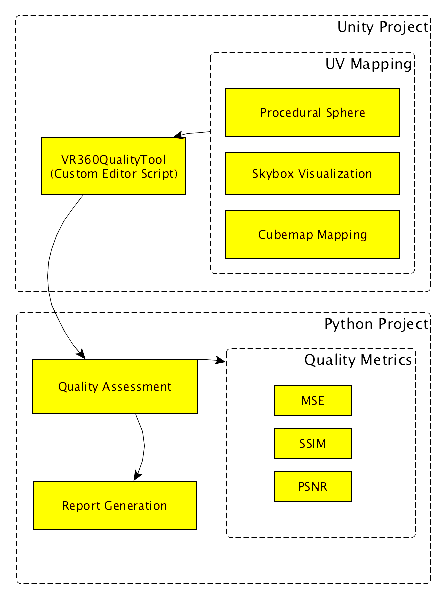
\includegraphics[width=0.9\linewidth]{tool_arch_en_edit.png}%
    \caption{Architecture of the proposed quality assessment tool.}
    \label{fig:fig_architecture}
\end{figure}

To make the user experience pleasant, an editor interface was developed in the form of a custom unity inspector, that is, a custom view of our component in C$\#$. In this component, users can define multiple preferences for the output image. These preferences include field of view angles, width and height as well as directions of the image to be created, comparison metrics to be used, and define whether graphs or a report will be generated at the end of the process. \par

Furthermore, the python layer is responsible for evaluating the pairs of images generated by the Unity layer. These images are evaluated using the scikit, numpy, and matplotlib libraries and the result of each metric is saved in a report at the end, which summarizes all the results.

\subsection{Qualitative and Quantitative Evaluation} \label{subsec:results}
%% Figures 0 %%

\begin{figure*}[!t]
    \centering

        \subfloat[Skybox 0;]{\includegraphics[width=0.24\linewidth]{{Screenshot_0_Skybox.jpg}}%
            \label{fig:skybox0}} \hfill
            \subfloat[Cubemap 0; ]{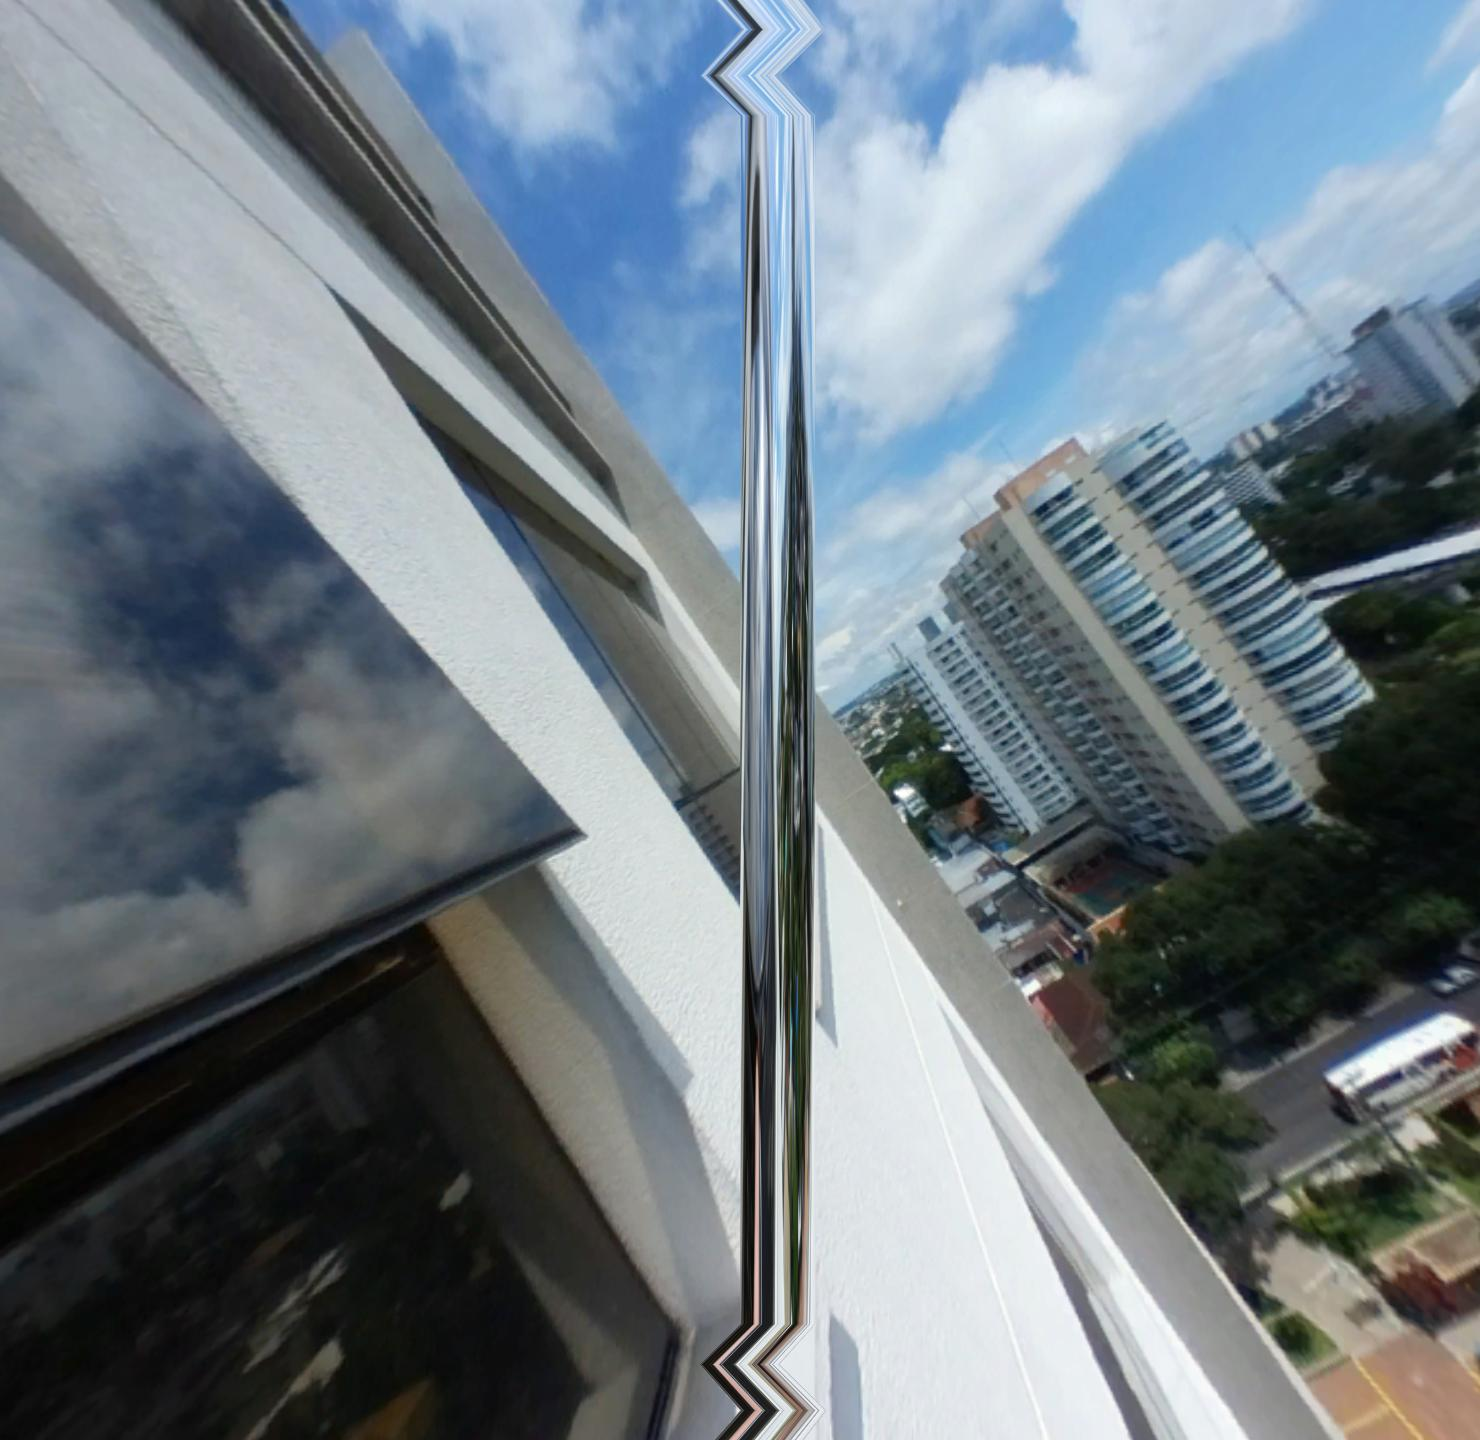
\includegraphics[width=0.24\linewidth]{Screenshot_0_Equi2Cube.jpg}%
            \label{fig:Cubemap0}} \hfill
        \subfloat[Sphere 0; ]{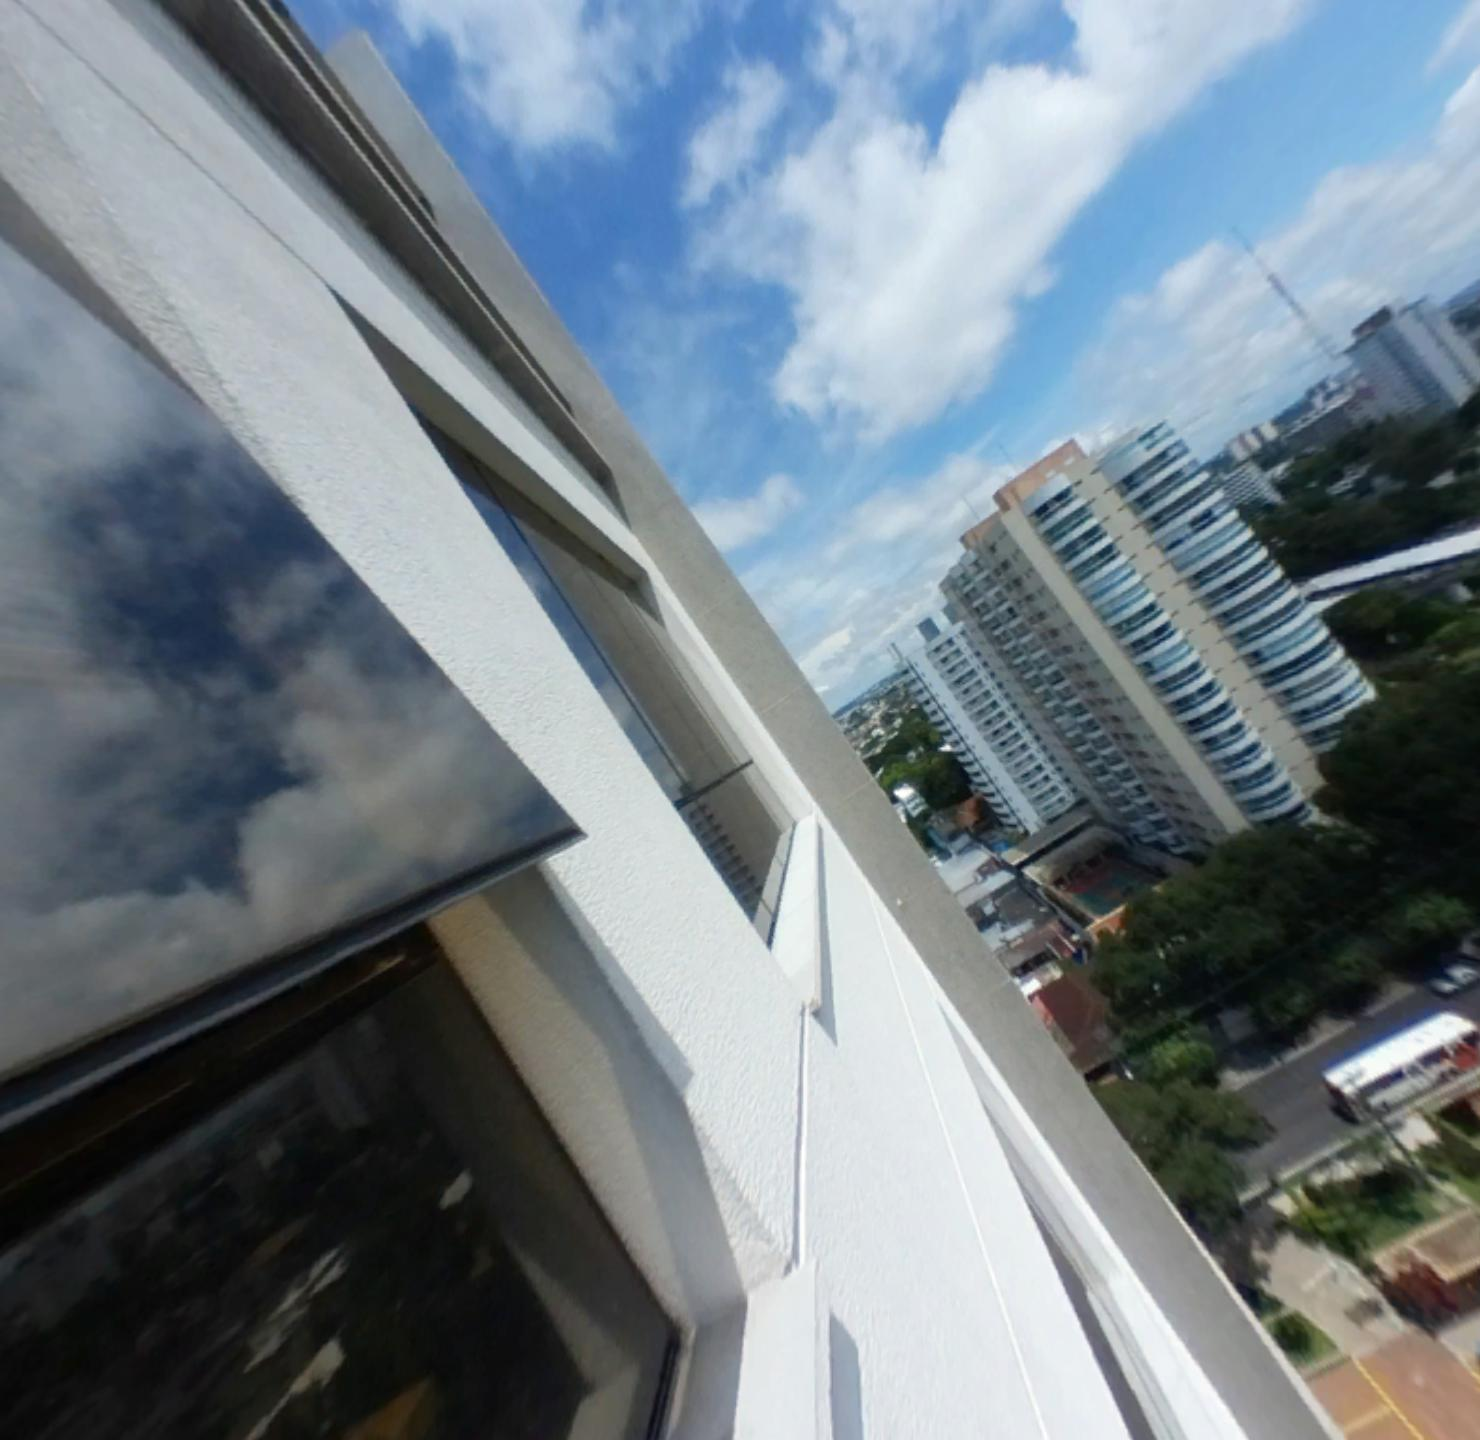
\includegraphics[width=0.24\linewidth]{Screenshot_0_Sphere.jpg}%
            \label{fig:Sphere0}} \hfill
            \subfloat[Cubemap (Error Corrected); ]{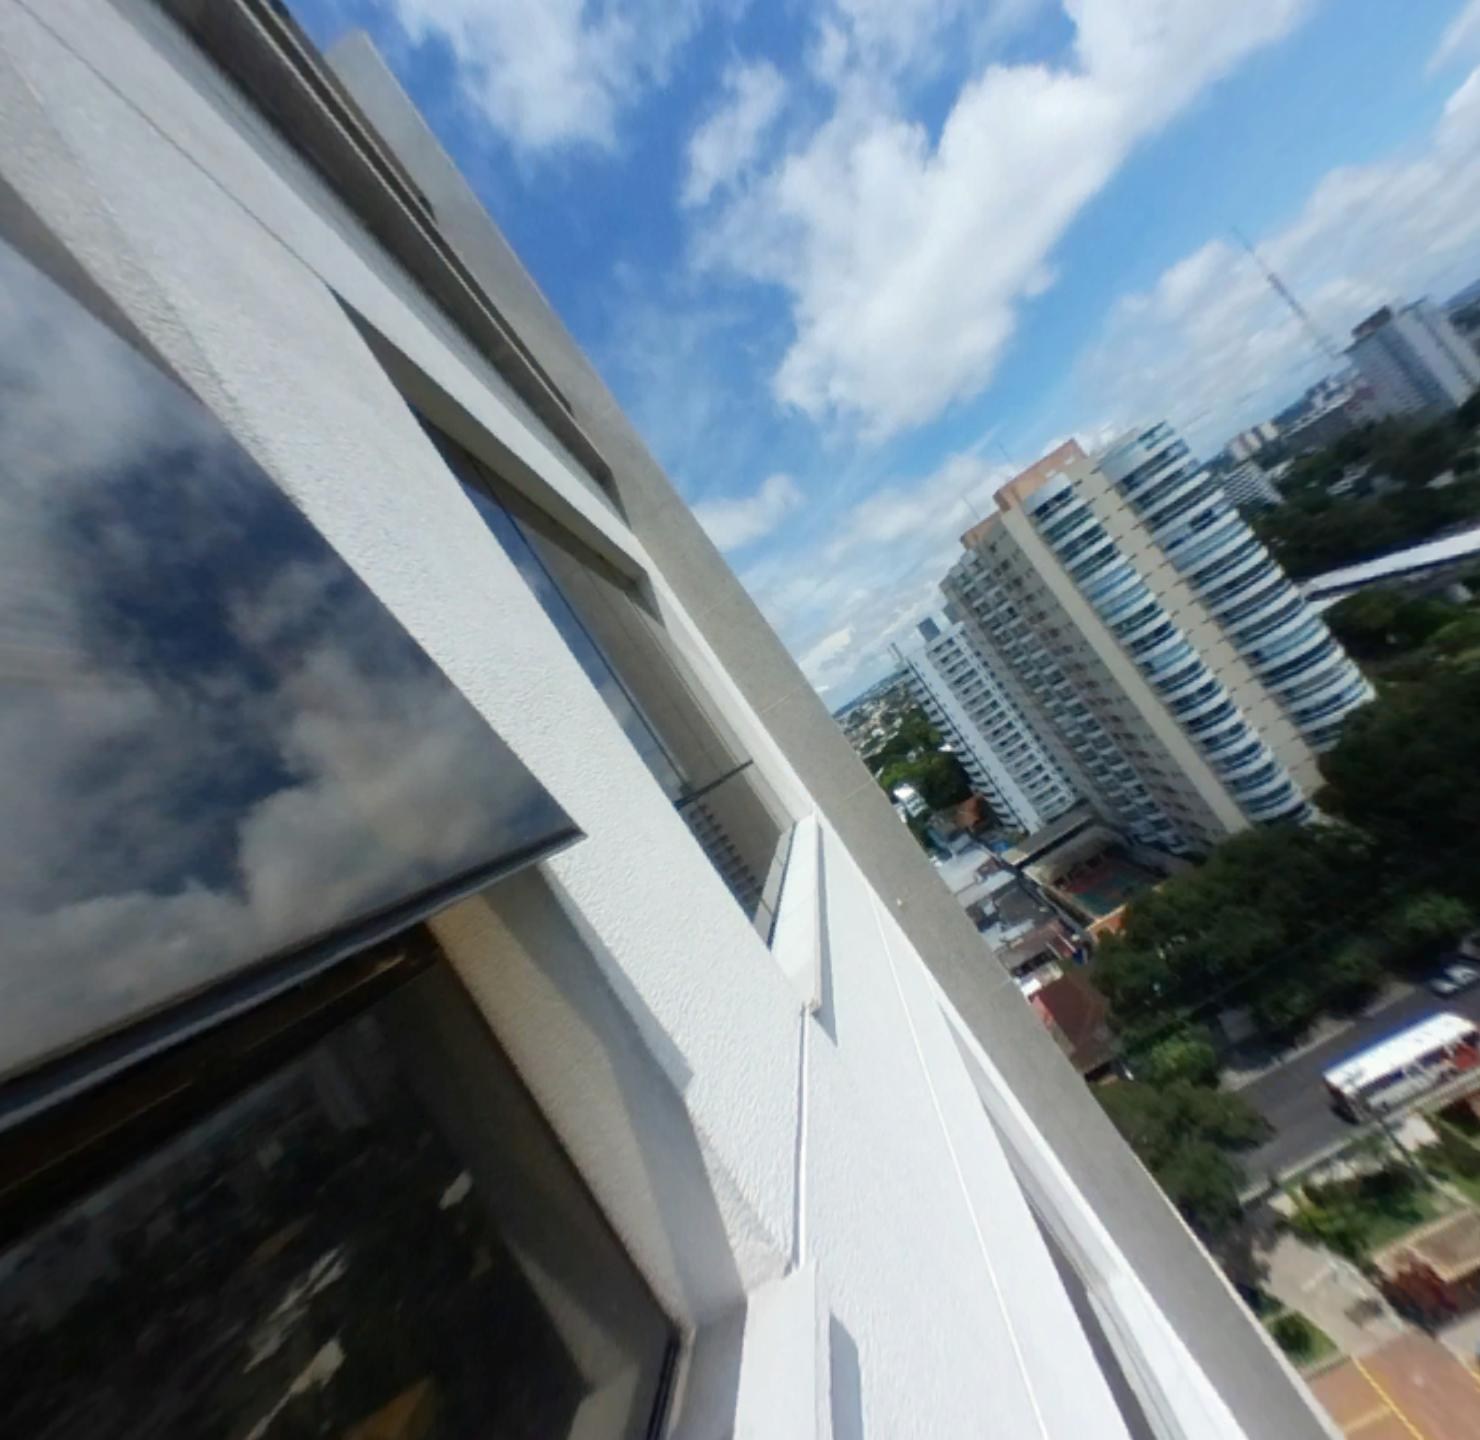
\includegraphics[width=0.24\linewidth]{figs/Screenshot_0_fixedEqui2Cube.jpg}%
            \label{fig:cubemap01}}
          \captionsetup{justification=centering}
    \caption{Example of images rendered in $D_0$ using: a) Skybox image is used as reference; b) result image rendered using cubemap; c) rendered using sphere.}
    \label{fig_examples1}
\end{figure*}

%% Figures 1 %%

\begin{figure*}[!ht]
    \centering

        \subfloat[Skybox 1;]{\includegraphics[width=0.24\linewidth]{{Screenshot_2_Skybox.jpg}}%
            \label{fig:skybox1}} \hfill
            \subfloat[Cubemap 1; ]{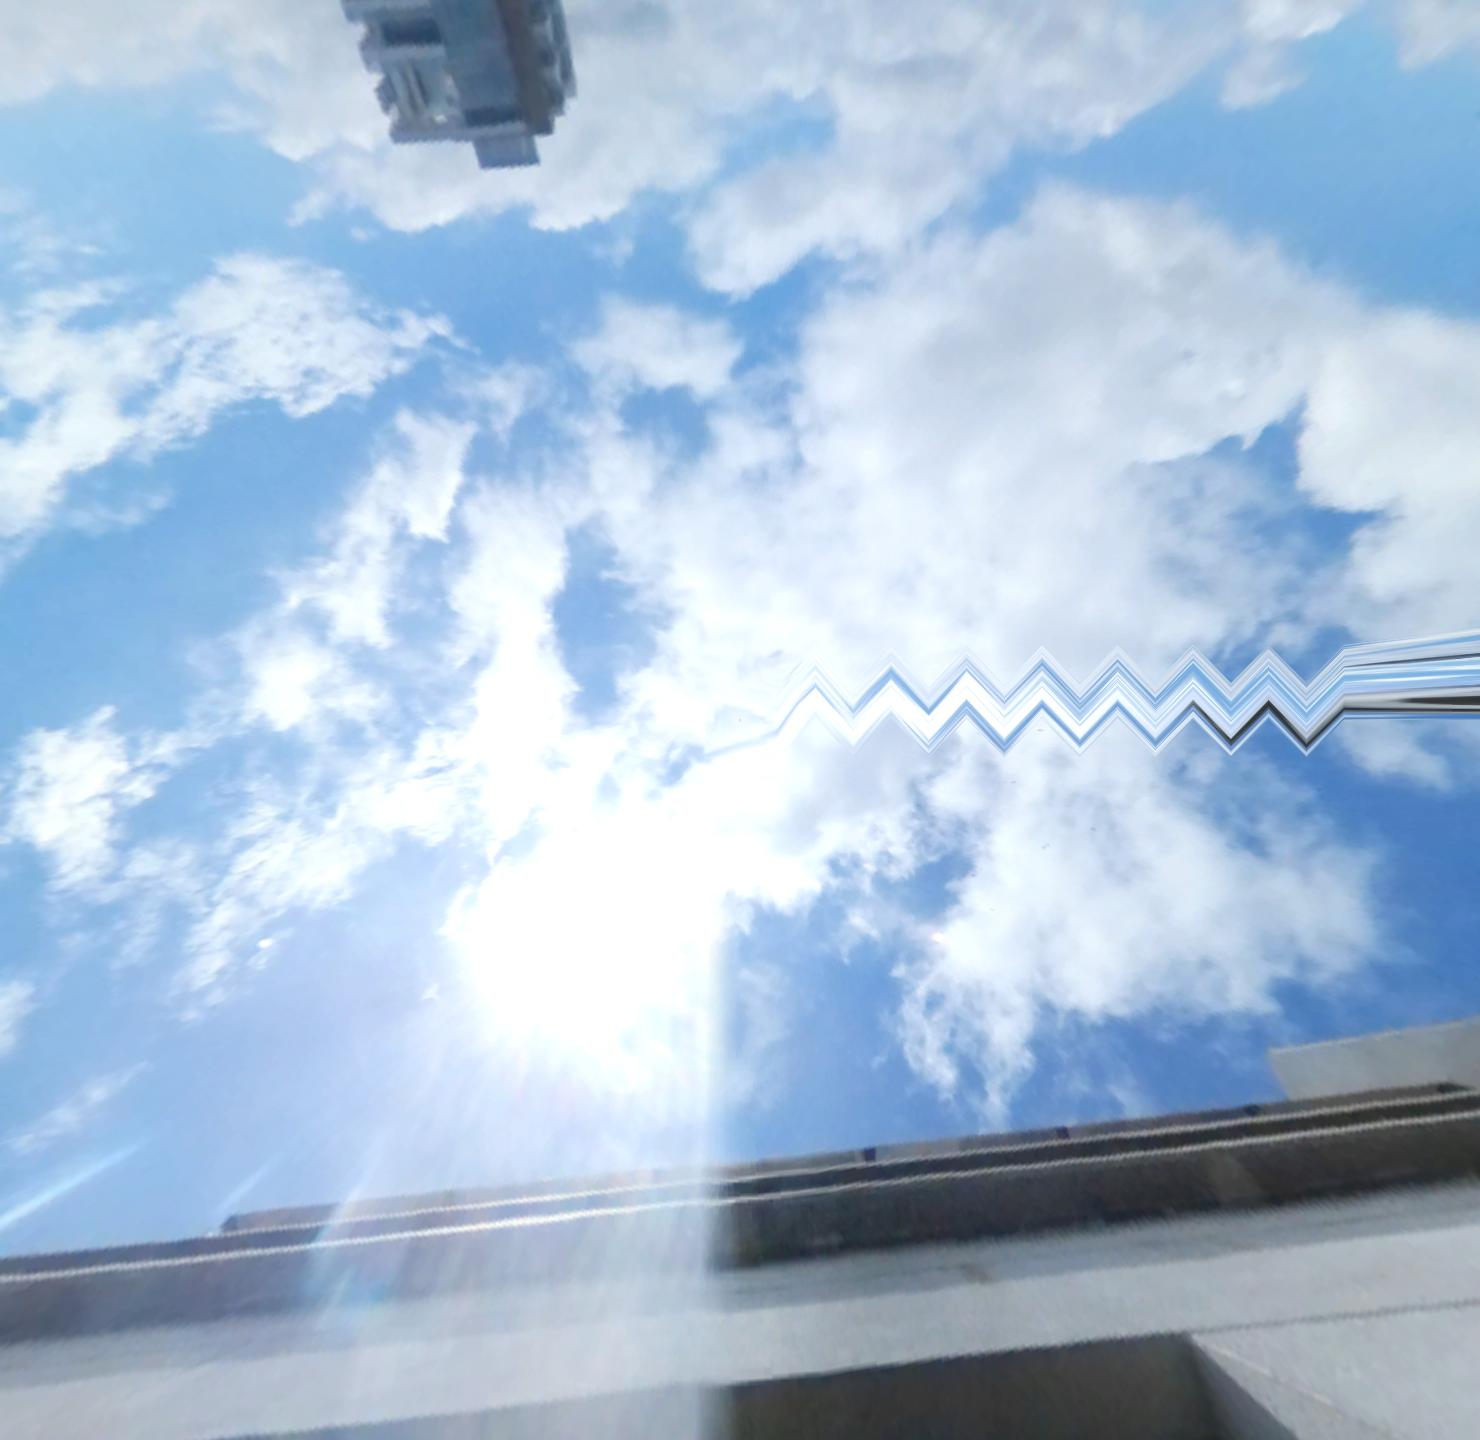
\includegraphics[width=0.24\linewidth]{Screenshot_2_Equi2Cube.jpg}%
            \label{fig:Cubemap1}} \hfill
        \subfloat[Sphere 1; ]{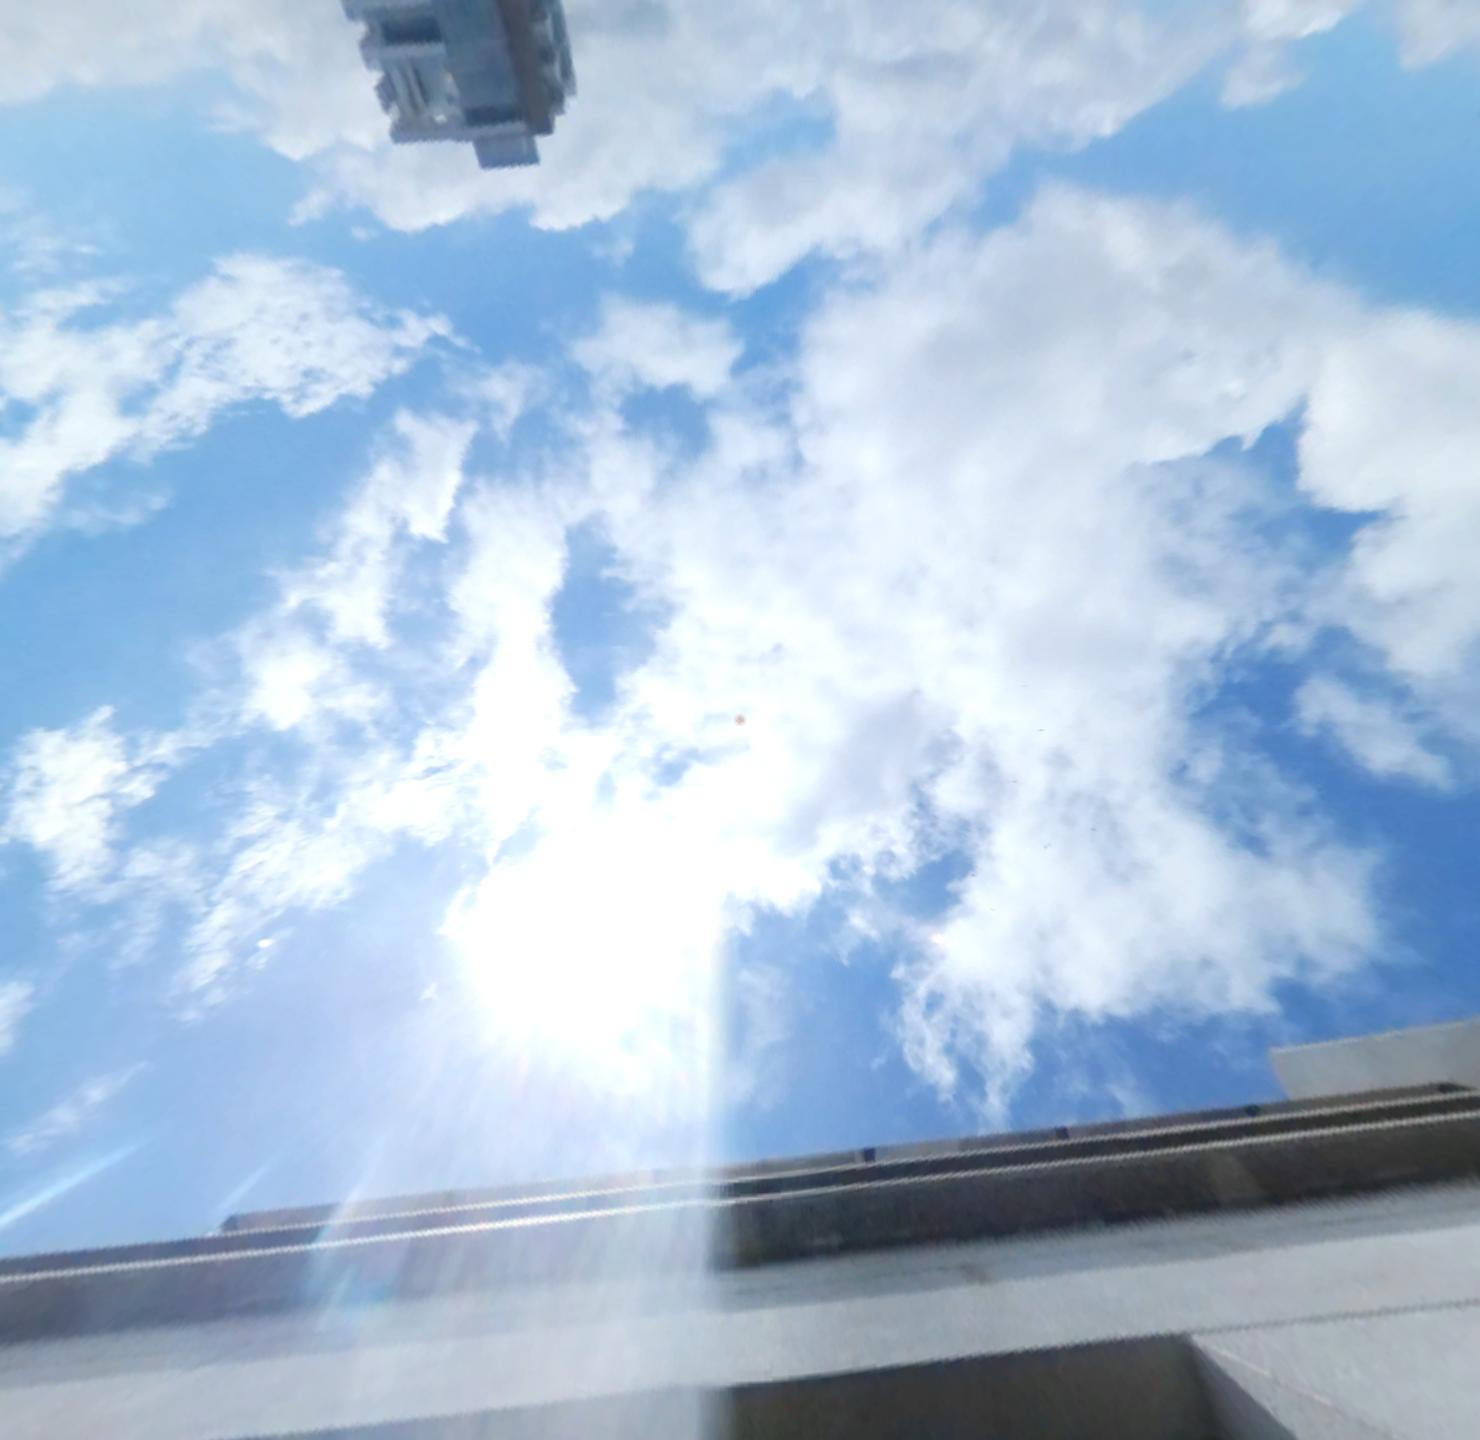
\includegraphics[width=0.24\linewidth]{Screenshot_2_Sphere.jpg}%
            \label{fig:Sphere1}} \hfill
            \subfloat[Cubemap (Error Corrected); ]{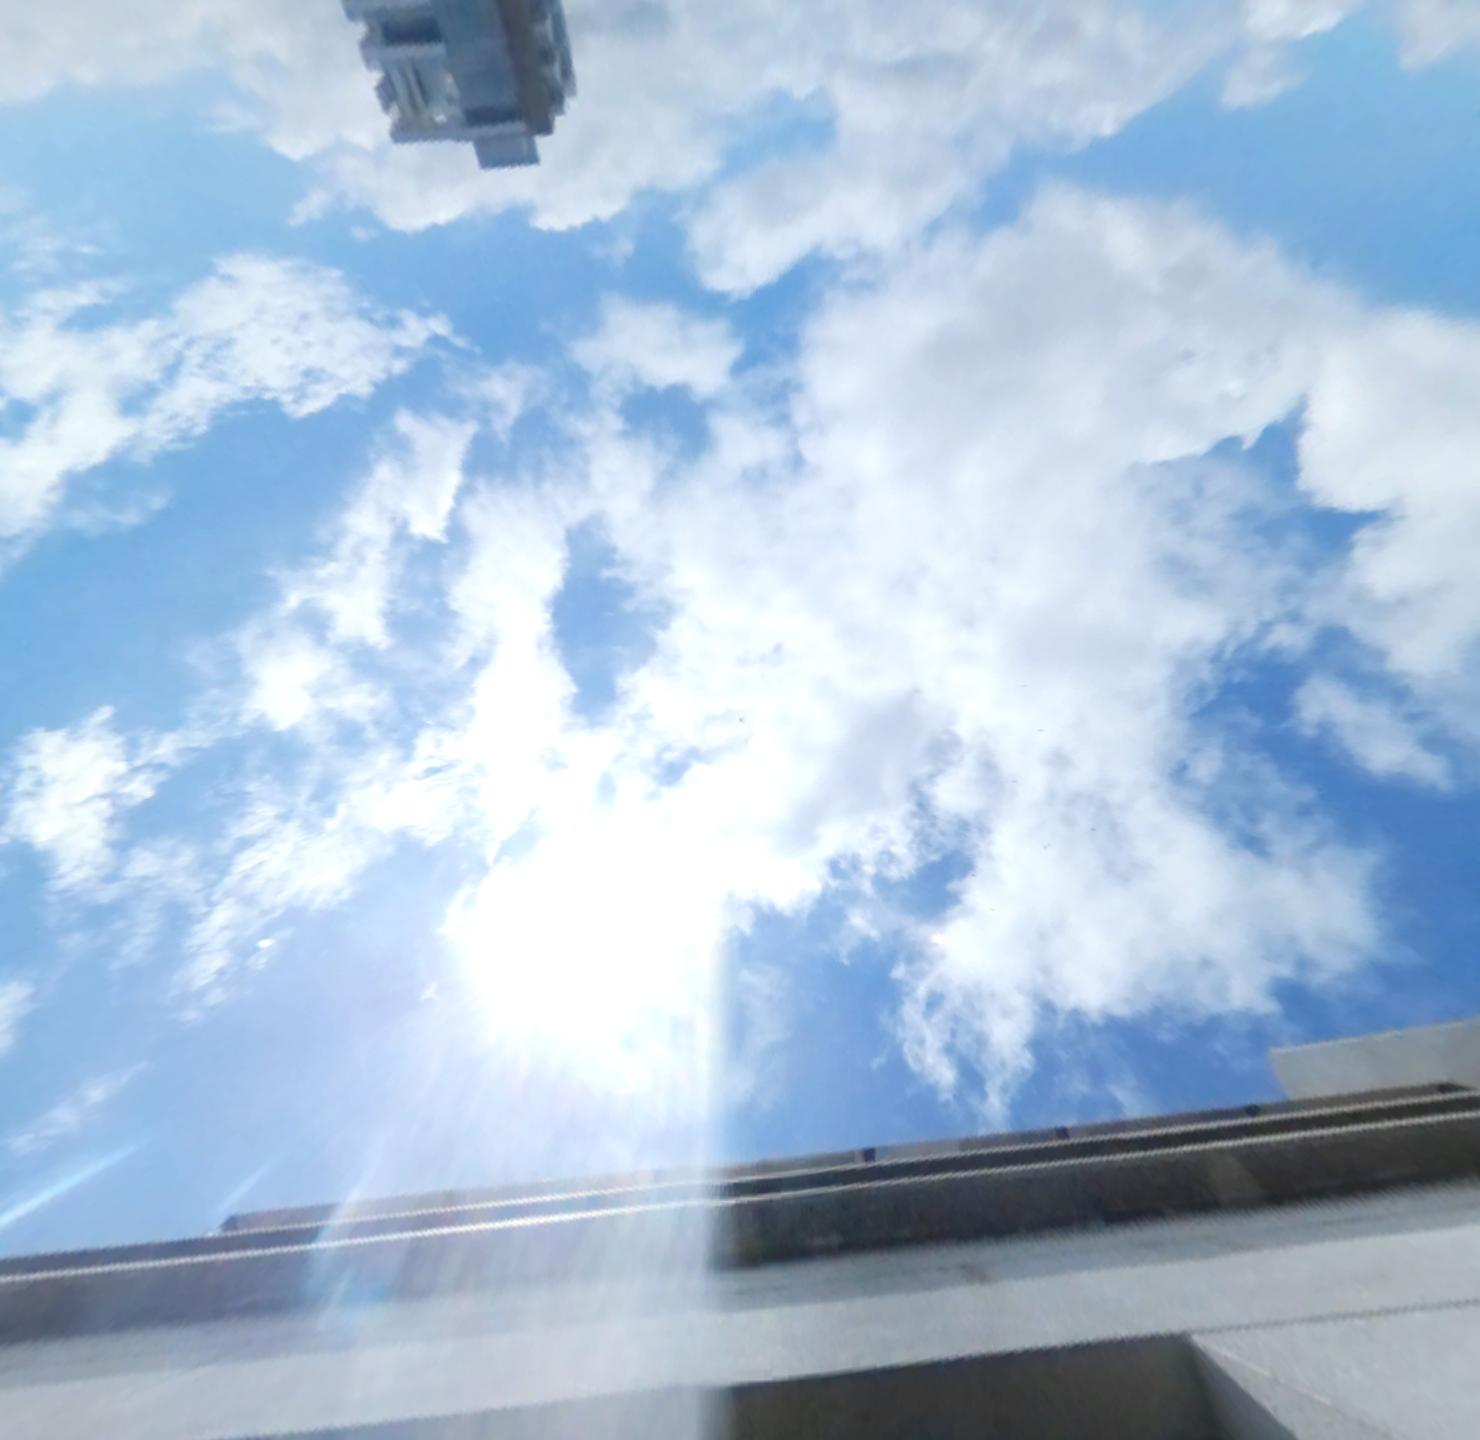
\includegraphics[width=0.24\linewidth]{figs/Screenshot_2_fixedEqui2Cube.jpg}%
            \label{fig:cubemap11}}
          \captionsetup{justification=centering}
    \caption{Example of images rendered in $D_1$ using: a) Skybox image is used as reference; b) result image rendered using cubemap; c) rendered using sphere.}
    \label{fig_examples3}
\end{figure*}

%% Figures 2 %%

%% Figures 5 %%
\begin{figure*}[!t]
    \centering

        \subfloat[Skybox 2;]{\includegraphics[width=0.24\linewidth]{{Screenshot_5_Skybox.jpg}}%
            \label{fig:skybox2}} \hfill
            \subfloat[Cubemap 2; ]{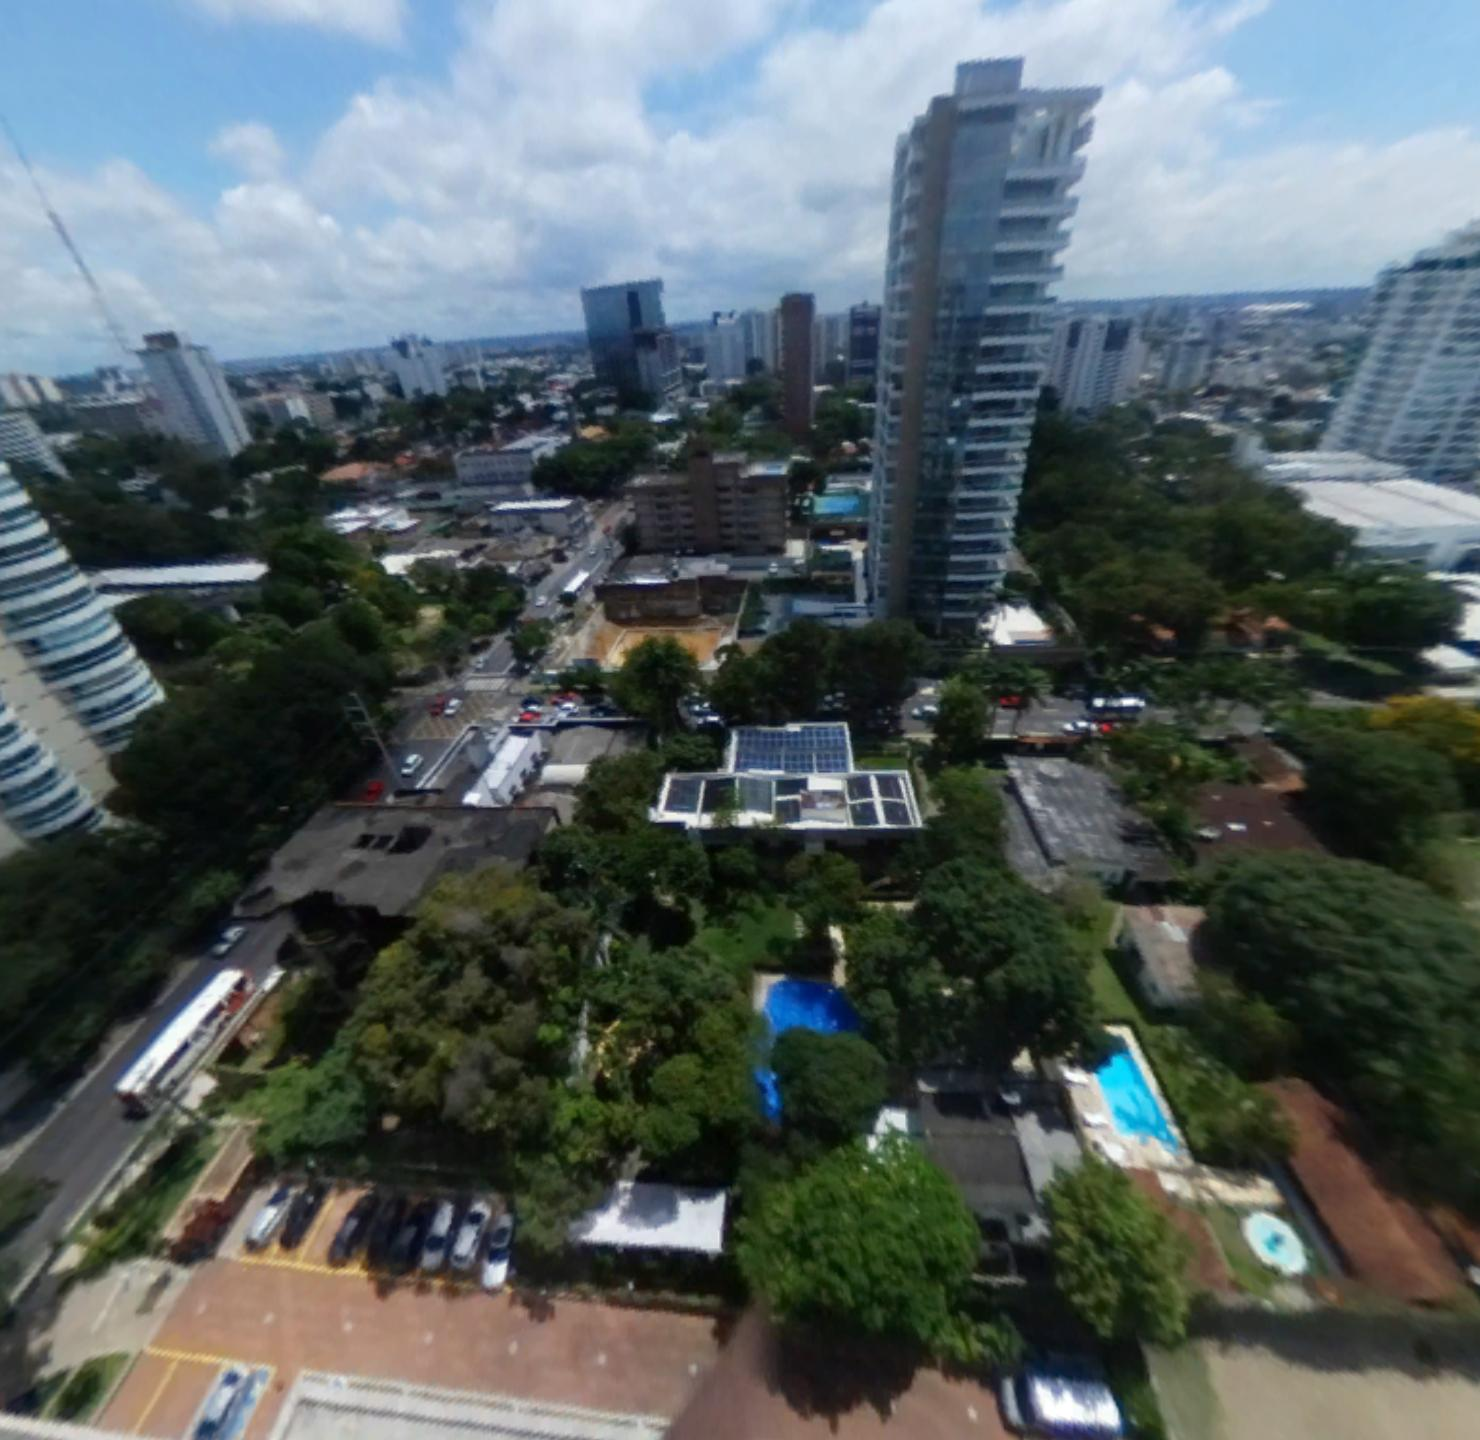
\includegraphics[width=0.24\linewidth]{Screenshot_5_Equi2Cube.jpg}%
            \label{fig:Cubemap2}} \hfill
        \subfloat[Sphere 2; ]{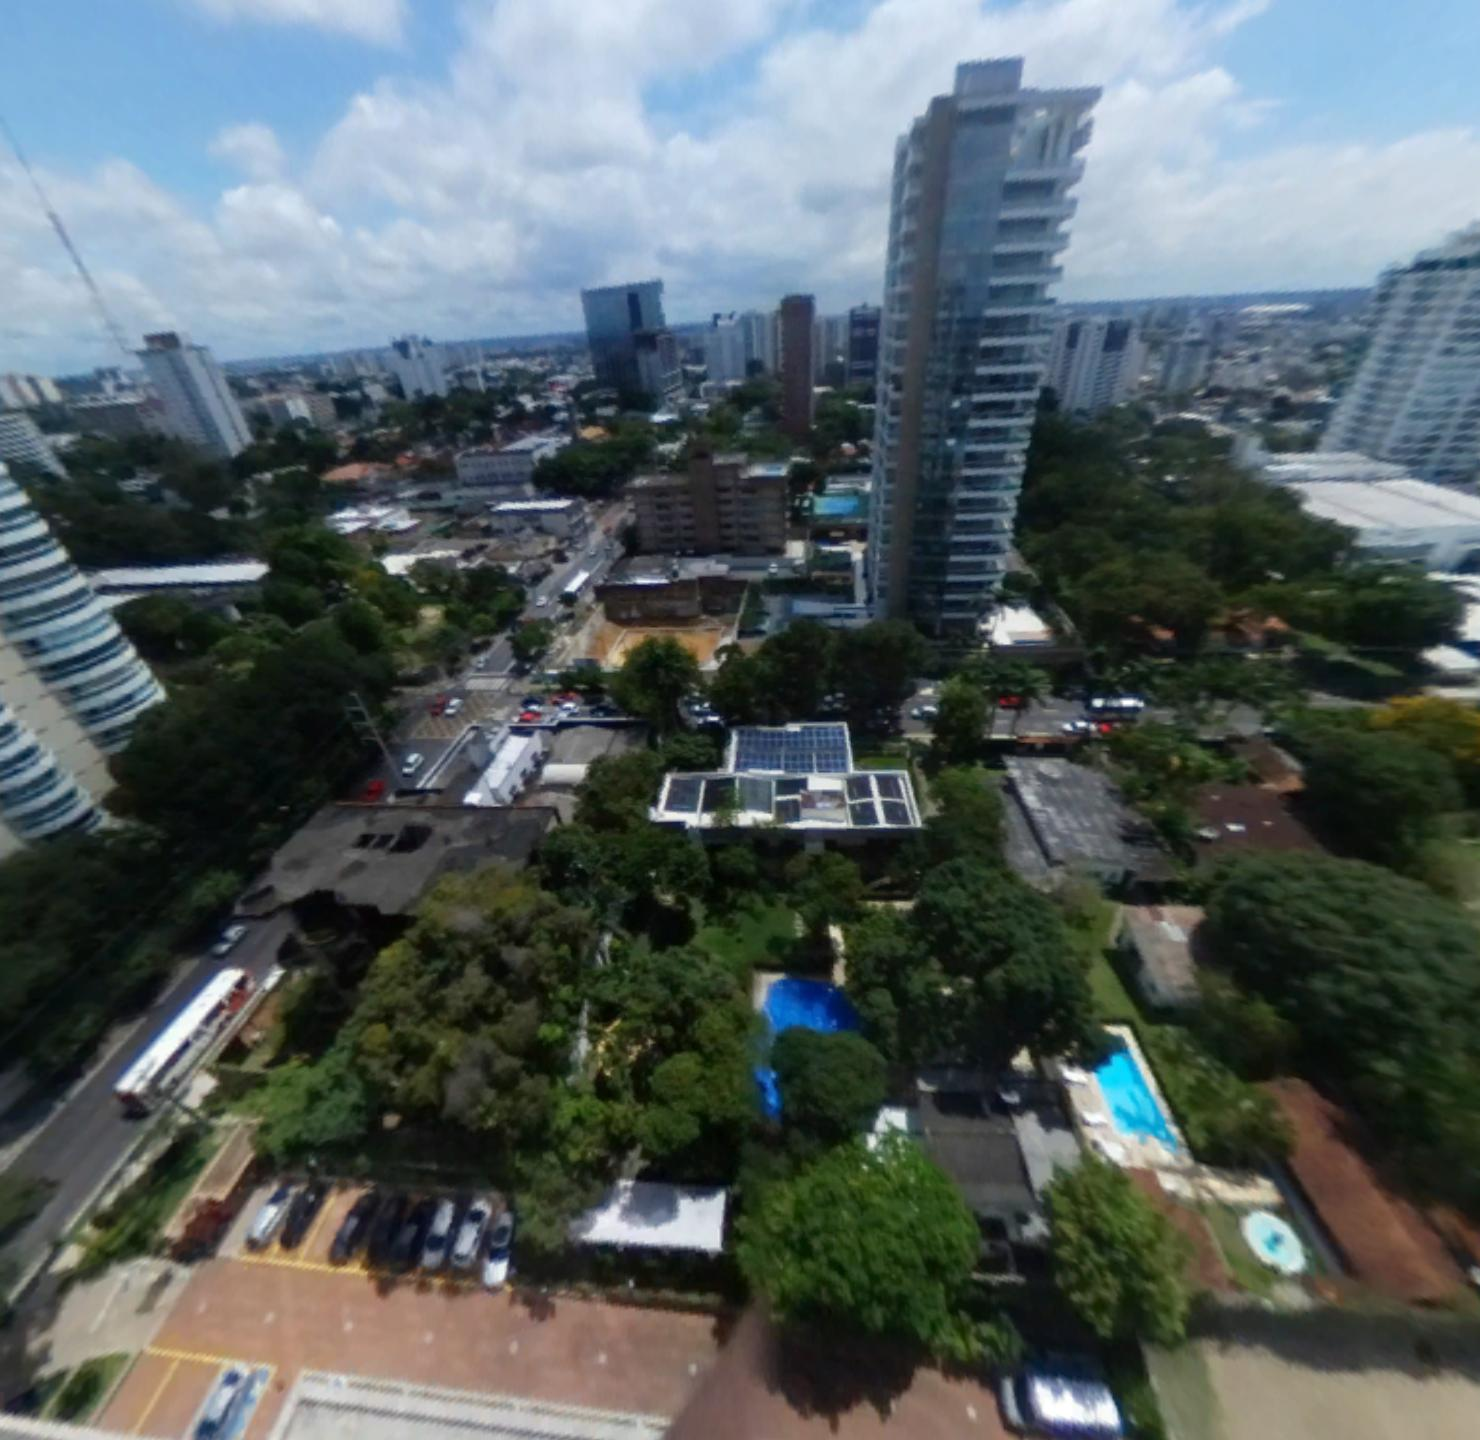
\includegraphics[width=0.24\linewidth]{Screenshot_5_Sphere.jpg}%
            \label{fig:Sphere2}} \hfill
             \subfloat[Cubemap (Error Corrected); ]{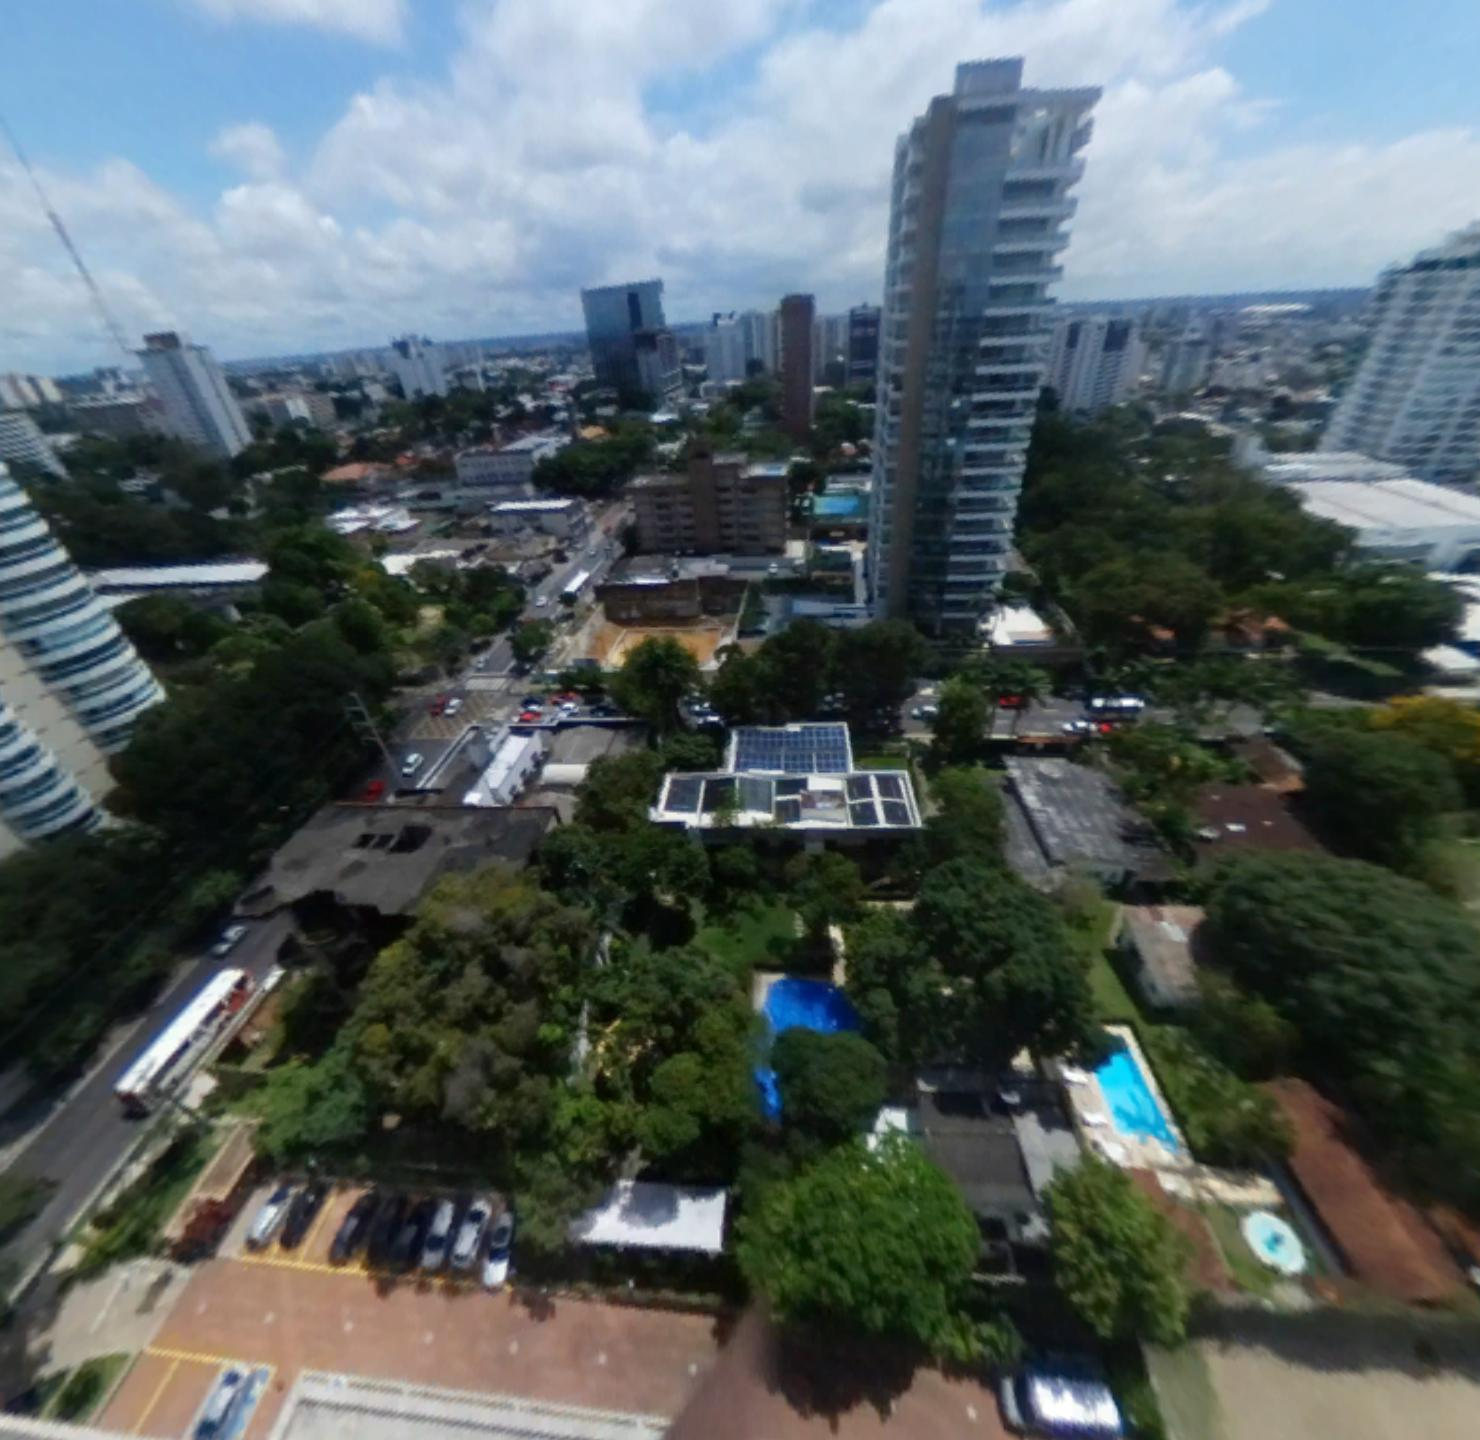
\includegraphics[width=0.24\linewidth]{figs/Screenshot_5_fixedEqui2Cube.jpg}%
            \label{fig:cubemap21}}
          \captionsetup{justification=centering}
    \caption{Example of images rendered in $D_2$ using: a) Cubmap image is used as reference; b) result image rendered using cubemap with error; c) rendered using sphere.}
    \label{fig_examples6}
\end{figure*}

The proposed tool was developed using Unity 2017.3.1F and python 2.7. This custom editor tool can be imported into any Unity project through a unitypackage, a standard format from Unity to distribute resources and tools. When adding VR360QualityTool script to a GameObject, the interface depicted at figure ~\ref{fig:tool} is presented. The field 'Screenshot Directions' allows to define one or more target directions, as explained in section ~\ref{sec:proposedMethod}. For our experiments, we used directions toward right $D_0 = (1.0, 0.0, 0.0)$, upside $D_1 = (0.0, 1.0, 0.0)$ and forward $D_2 = (1.0, 0.0, -1.0)$, respectively. Each direction can be visualized in figures~\ref{fig_examples1},~\ref{fig_examples3} and~\ref{fig_examples6}.

\begin{table*}[!t]
 \centering
    \caption{Metrics Results Example}
       \label{table_metrics}
       \resizebox{0.8\textwidth}{!}{
        \begin{tabular}{c|ccc|ccc|ccc}
            \hline
            \rule{0pt}{1.05em} % juju's magic trick to set top spacing
            & \multicolumn{3}{c|}{Direction 0}
            & \multicolumn{3}{c|}{Direction 1}
            & \multicolumn{3}{c}{Direction 2}
            \\
        \hline
        \rule{0pt}{1.1em} % juju's magic trick to set top spacing
            % & \begin{tabular}{c|c c|c c|c c}
            % & \multicolumn{2}{c|c|c}{Cubemap Sphere} \\
                    & $S$ & $C_e$ & $C_f$& $S$ & $C_e$ & $C_f$& $S$ & $C_e$ & $C_f$ \\
            MSE     & $50.27$ & $551.27$ & $1.29$& $39.99$ & $41.89$ & $0.70$& $27.88$ & $18.60$ & $2.40$ \\
            % \hline
            SSIM    & $0.93$ & $0.93$ & $0.99$& $0.93$ & $0.97$ & $1.00$& $0.87$ & $0.96$ & $0.99$ \\
            % \hline
            PSNR    & $31.12$ & $20.72$ & $47.01$& $32.11$ & $31.91$ & $49.66$& $27.88$ & $35.43$ & $44.33$ \\
            \hline
            % \end{tabular}
        \end{tabular}
    }
\end{table*}

Different rendering approaches were used in our experiments: Skybox (used as reference), a sphere-based shader ($S$), a cubemap shader ($C_e$) with an interpolation error, and a normal cubemap shader ($C_f$). The distorted cubemap was created intentionally to prove our method is capable of identifying such errors. It occurs in triangles which have UV coordinates between 0.9 to 0.1. Instead of interpolating to the chosen direction, this cubemap interpolates to the opposite direction (0.7, 0.6 ... 0.1, x) and compresses the whole image in a tight image region. Both cubemap implementations are employing equirectangular conversion as explained at subsection~\ref{subsec:equiconvtocubemap}.


To perform the quality assessment each image is compared to its respective direction in the reference image. Figures ~\ref{fig:skybox0}, ~\ref{fig:skybox1} and ~\ref{fig:skybox2} are produced by Skybox rendering which is used as reference for each evaluated direction. The skybox rendered image patch is compared with those obtained with the spherical rendering $S$ in figure~\ref{fig:Sphere0}, with cubemap rendering $C_e$ \textcolor{red}{which contains interpolation error} in figure~\ref{fig:Cubemap0} and with cubemap rendering $C_f$ in figure~\ref{fig:Cubemap1}.  Figures~\ref{fig_examples1},~\ref{fig_examples3} and ~\ref{fig_examples6} shows all images used as input for our proposed evaluation system and their results can be seen at table ~\ref{table_metrics}.

%% Table Results %%

% \begin{table}[h!]
% \caption{Metrics Results}
%       \label{table_metrics}
% \resizebox{0.5\textwidth}{!}{
%     \begin{tabular}{c c c c}
%     \hline
%     Metrics & MSE & SSIM & PSNR \\
%     \hline
%     Direction 0 - Cubemap & $551.27$ & $0.93$ & $20.72$ \\
%     \hline
%     Direction 1 - Cubemap & $41.89$ & $0.97$ & $31.91$ \\
%     \hline
%     Direction 2 - Cubemap & $18.60$ & $0.96$ & $35.43$ \\
%     \hline
%     Direction 0 - Sphere & $0.00$ & $1.00$ & $100.00$ \\
%     \hline
%     Direction 1 - Sphere & $0.00$ & $1.00$ & $100.00$ \\
%     \hline
%     Direction 2 - Sphere & $0.00$ & $1.00$ & $100.00$ \\
%     \hline
%     \end{tabular}
%     }
% \end{table}

After processing the images, the results are summarized in the generated report, as demonstrated by the table~\ref{table_metrics}. Cubemap $C_f$ rendering approach had the best results in all directions for all metrics. Since the UV mapping of Skybox rendering is similar to the UV mapping of the cubemap approach, they tend to generate more similar images for a same direction. In contrast to this, cubemap $C_e$ presents a very noticeable distortion region for directions $D_0$ and $D_1$ as depicted in figures ~\ref{fig:Cubemap0} and ~\ref{fig:Cubemap1}. As a result the MSE value for both directions are very degraded. Thus we can conclude that MSE, SSIM and PSNR are good enough to identify images patches with shader errors given a reasonable reference image.

Despite the absence of rendering errors in the sphere shader $S$, its metrics values are surpassed by the cubemap $C_f$. This is explained by the difference between the distortions of a sphere-based and a Skybox-based rendering. The equirectangular mapping requires a sinusoidal UV mapping. Considering that the sphere has a sinusoidal mapping in its vertices,  the UV coordinates are interpolated linearly inside each triangle. On the other hand, skybox mapping employs a sinusoidal mapping inside the pixel shader and consequently affects every pixel produced. However, for the end-user, such differences are not perceptually remarkable.

After every iteration, our tool presents the metrics, for example, the table ~\ref{table_metrics}. The best rendering candidates are ranked based on their performance in each metric and direction.

\section{Conclusion}\label{sec:conclusion}

We proposed the development of an equirectangular image quality assessment tool which uses objective metrics such as MSE, SSIM and PSNR in order to facilitate choosing among different image resolutions and mapping solutions.

Our tool is integrated into the Unity Editor as Unity is the most used development engine for virtual reality applications. Different UV mapping techniques were used to visualize 360\degree images: latitude/longitude in a inverted sphere; skybox; and cubemap. We also demonstrated how to convert a equirectangular image into a cubemap texturing using a custom shader.

This Unity implemention assess image quality of already implemented rendering approaches for equirectangular image visualization. Full-reference objective metrics are applied.

One of the limitation of our tool is that the user needs to simulate the target device, by emulating a specific resolution and field view. For future work, we plan to obtain directly from rendering on the mobile devices where VR applications can be executed. Thus, we also plan an embedded component in the application that allows you to reap results while running the application on the mobile device. We also envisage to conduct subject evaluations in order to pick better metrics for quality assessment of image patches.

% conference papers do not normally have an appendix

% use section* for acknowledgment
\section*{Acknowledgment}
The authors would like to thank the support provided by SIDIA Instituto de Ciência e Tecnologia and teams.

\bibliographystyle{IEEEtran}
\bibliography{equitool_sibgrapi19}
\end{document}


